\section{Příklad 3}
% Jako parametr zadejte skupinu (A-H)
\tretiZadani{B}

\vspace{1cm}
\large{\textbf{Rešení (Metoda uzlových napětí):}}
\vspace{0.5cm}

%%% Krok 1
\begin{center}
\textbf{Krok 1} - Vyznačíme si proudy a vytvoříme si rovnice pro uzly A, B, C. \\
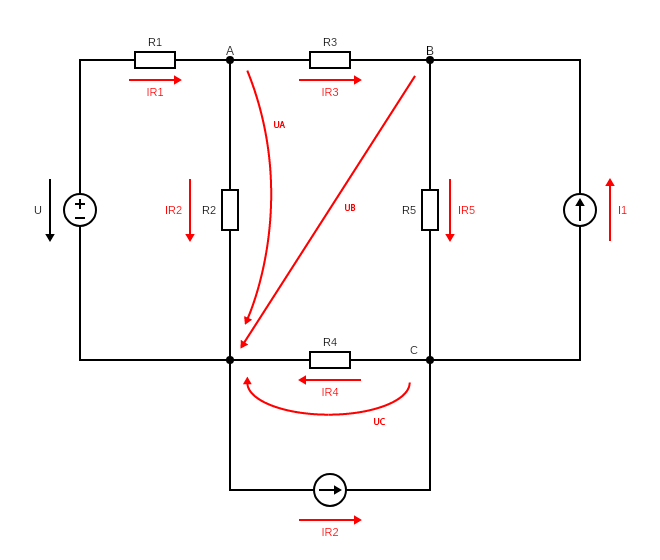
\includegraphics[scale=0.35,keepaspectratio]{fig/Pr3_steps/Pr3_step01.png}
\end{center}
\vspace{-0.5cm}

\begin{gather*}
A: I_{R_1} - I_{R_3} - I_{R_2} = 0 \\\\
\newline
\newline
B: I_{R_3} + I_1 - I_{R_5} = 0 \\\\
\newline
\newline
C: I_2 - I_1 + I_{R_5} - I_{R_4} = 0
\end{gather*}

\newpage

%%% Krok 2
\begin{center}
\textbf{Krok 2} - Pomocí Ohmova zákona vyjadříme rovnice pro jednotlivé proudy. \\
\end{center}

\begin{gather*}
I_{R1} = \frac{U - U_A}{R_1} \\\\
\newline
\newline
I_{R2} = \frac{U_A}{R_2} \\\\
\newline
\newline
I_{R3} = \frac{U_A - U_B}{R_3} \\\\
\newline
\newline
I_{R4} = \frac{U_C}{R_4} \\\\
\newline
\newline
I_{R5} = \frac{U_B - U_C}{R_5} \\\\
\end{gather*}

%%% Krok 3
\begin{center}
\textbf{Krok 3} - Dosdíme do rovnic pro uzly A, B, C. \\
\end{center}

\begin{gather*}
\frac{U - U_A}{R_1} - \frac{U_A - U_B}{R_3} - \frac{U_A}{R_2} = 0\\\\
\newline
\newline
\frac{U_A - U_B}{R_3} + 0,7 - \frac{U_B - U_C}{R_5} = 0 \\\\\
\newline
\newline
0,8 - 0,7 + \frac{U_B - U_C}{R_5} - \frac{U_C}{R_4} = 0 \\\\
\end{gather*}

\newpage


%%% Krok 4
\begin{center}
\textbf{Krok 4} - Rovnice pro uzly převedeme do matice a vypočítáme pomocí Cramerova a Sarussova pravidla. \\
\end{center}

\begin{gather*}
    \begin{pmatrix}
        \frac{-1}{R_1}+\frac{-1}{R_3}+\frac{-1}{R2}&\frac{1}{R_3} & 0 \\\\
        \frac{1}{R_3}&\frac{-1}{R_3}+\frac{-1}{R_5}  & \frac{1}{R_5} \\\\
        0&\frac{1}{R_5} &\frac{-1}{R_3}+\frac{-1}{R_5}
    \end{pmatrix}
    \times
    \begin{pmatrix}
        U_A \\\\
        U_B \\\\
        U_C
    \end{pmatrix}
    =
    \begin{pmatrix}
        -3,0612 \\\\
        -0,7 \\\\
        -0,1
    \end{pmatrix}
\end{gather*}

\vspace{0.75cm}

\begin{gather*}
    \begin{pmatrix}
        \frac{-1}{49}+\frac{-1}{61}+\frac{-1}{45}&\frac{1}{61} & 0 \\\\
        \frac{1}{61}&\frac{-1}{61}+\frac{-1}{34}  & \frac{1}{34} \\\\
        0&\frac{1}{34} &\frac{-1}{61}+\frac{-1}{34}
    \end{pmatrix}
    \times
    \begin{pmatrix}
        U_A \\\\
        U_B \\\\
        U_C
    \end{pmatrix}
    =
    \begin{pmatrix}
        -3,0612 \\\\
        -0,7 \\\\
        -0,1
    \end{pmatrix}
\end{gather*}

\vspace{0.5cm}

\begin{gather*}
U_A = 68,6069 V \\\\
\newline
\newline
U_B = 60,2811 V \\\\
\newline
\newline
U_C = 31,8406 V
\end{gather*}

\vspace{1cm}

%%% Krok 5
\begin{center}
\textbf{Krok 5} - Vypočítáme $I_{R_2}$ a $U_2$. \\
\end{center}

\begin{gather*}
\boldsymbol{I_{R_2}} = \frac{U_A}{R_2} = \frac{68,6069}{45} = \boldsymbol{1.5246 A} \\\\
\newline
\newline
\boldsymbol{U_2} = U_A = \boldsymbol{68,6069 V}
\end{gather*}